\documentclass[11pt, a4paper, preprint]{article}

\usepackage{amsmath, amssymb, graphicx, outline, float, cite, color}
\usepackage{longtable,array}
\renewcommand{\thefigure}{S\arabic{figure}}
\renewcommand{\thetable}{S\arabic{table}}

\usepackage[T1]{fontenc}
\usepackage[utf8]{inputenc}
\usepackage{authblk}
\newcommand{\tcr} { \textcolor{red} }


\title{Supplementary Materials for \\
Modeling the competing effects of the immune system and EMT on epithelial cancers
}
\author{Daniel R. Bergman$^{1}$,
Matthew Karikomi\,$^{1}$,
Qing Nie\,$^{1,2,*}$
and \\Adam L. MacLean\,$^{3,*}$
}
\affil{
  $^1$Department of Mathematics, University of California, Irvine,  Irvine, CA 92697, USA \\
  $^2$Department of Cell and Developmental Biology, University of California, Irvine, Irvine, CA 92697, USA \\
  $^3$Department of Biological Sciences, University of Southern California, Los Angeles, CA 90089, USA \\
  $^*$Correspondence:  qnie@uci.edu (Q.N.); macleana@usc.edu (A.L.M.)
}
\renewcommand\Authands{ and }

\date{}

\begin{document}
\maketitle
\tableofcontents
\listoftables
\listoffigures

\section{Model Description}

\subsection{Tissue cell fate}
During each cell cycle, every cell randomly is assigned a cell fate from the following options:
\begin{itemize}
\item proliferation
\item apoptosis
\item immune clearance (by NKs or CTLs)
\item rest in $G_0$
\end{itemize}

For each cell, a weight is chosen for each option and these are normalized to probabilities which then are used to randomly determine what each cell does during the cell cycle.

\subsubsection{Proliferation}
There are four factors that contribute to the weight of a cell to proliferate.
The first is a base proliferation rate that all cells have, $p$.
Second, if the cell has a mutation in the proliferation pathway ($\delta_P=1$), then the weight for proliferation is proportionally increased by $\Delta_P$.
Third, if the cell is mesenchymal ($\zeta=1$), then the weight for proliferation is proportionally decreased by $\Delta_{\text{MGA}}$, which stands for mesenchymal growth arrest.
This lost proliferation for mesenchymal cells will later be used to increase their chance of resting.
Fourth, there is a negative feedback of the cells on their own proliferation which is quantified by a Hill factor as a function of the tissue cell population, $N_C$, with EC50 term $K_0$.
In total, the weight for proliferation is given by

\begin{equation}\tag{2.1}
\rho_P = p(1+\delta_{P}\Delta_P)(1-\zeta \Delta_{\text{MGA}})\frac{K_0}{K_0+N_C}
\end{equation}

\subsubsection{Apoptosis}
There are two factors that contribute to a cell's weight for undergoing apoptosis.
There is a basal apoptosis rate that all cells experience, $d_C$ for death.
Second, if the cell has a mutation in the apoptosis pathway ($\delta_A=1$), then the weight for undergoing apoptosis is proportionally decreased by $\Delta_A$.
In total, the weight for apoptosis is given by 

\begin{equation}\tag{2.2}
\rho_A = d_C(1-\delta_{A}\Delta_A)
\end{equation}

\subsubsection{Immune Clearance}
For both NK clearance and CTL clearance, the weights are built with the same factors but have different parameter values for NK and CTLs.
First of all, the cell needs to be malignant ($\delta_{\text{MUT}}=1$).
Second, there is a Hill factor that captures the probability of an immune cell finding and interacting with the given tissue cell with EC50 term $K_1$.
Third, NKs and CTLs have their own efficacy parameters, $E_{\text{NK}}$ and $E_{\text{CTL}}$, which can be understood as the rate of immune clearance given an immune cell has found the mutated cell.
Fourth, there is a decreasing Hill factor based on the number of Treg cells present with EC50 term $K_2$.
Finally, there are two factors that proportionally decrease the weight of immune clearance depending on if the cell has an immune evasion mutation ($\delta_{\text{IE}}=1$) or if it is mesenchymal ($\zeta=1$) with respective decreases $\Delta_{\text{IE}}$ and $\Delta_{\text{MIE}}$.
In total, the weight of NK clearance is given by

\begin{equation}\tag{2.3}
\rho_{\text{NK}} =\delta_{\text{MUT}} \frac{N_{\text{NK}}}{N_C/K_{1}+N_{\text{NK}}}  \frac{E_{\text{NK}}}{1+N_{\text{Treg}}/K_2} (1-\delta_{\text{IE}}\Delta_{\text{IE}})(1-\zeta \Delta_{\text{MIE}})
\end{equation}

A similar formula holds for CTLs with only the number of CTLs and their efficacy being different from the above equation.


\subsubsection{Rest in $G_0$} 
The weight associated with rest is taken as 1 except in the case of mesenchymal cells.
Recall that mesenchymal cells had their proliferation rate decreased by $1-\zeta\Delta_{\text{MGA}}$ (see Eq. 2.1).
The biological assumption here is that mesenchymal cells instead of proliferating will instead rest, so this lost proliferation weight is added to the resting weight.
Hence, the weight of rest is given by

\begin{equation}\tag{2.4}
\rho_R = 1 + \zeta p(1+\delta_P\Delta_P)\Delta_{\text{MGA}}\frac{K_0}{K_0+N_C}
\end{equation}

Again, the reason for adding that term is due to the understanding that overall mesenchymal cells proliferate less as individual cells rest longer in the $G_0$ phase.

\subsubsection{Completing the Cell Cycle}
After the cell fates are determined and the results reflected in the system, there are a few things that happen before the system moves on to a new cell cycle.
First, the NK and CTL populations are reduced by the number of mutated cells they cleared.
This represents the fact that individual immune cells lose efficacy as they carry out their effector functions. 
Second, all proliferating cells have a cell-specific probability of undergoing a driver mutation in one of the three pathways.
If they do, one is randomly chosen among the three pathways and the pathway in that cell becomes altered.
If the cell does not undergo a mutation, then its probability of mutation during subsequent cell cycles increases.
\par
Finally, the EMT values for each cell is updated.
This depends on the cells current EMT score and how much TGF-$\beta$ is currently in the system.
The amount of TGF-$\beta$ absorbed by all cells is given by an increasing Hill function in terms of the TGF-$\beta$ in the TME.
The saturation effect is to limit the amount of TGF-$\beta$ a cell can absorb in a given time interval.
This quantity is then divided up randomly among the $N_C$ living cells via a normally distributed noise term to determine how much exogenous TGF-$\beta$ each cell receives during this cell cycle.
Should this value, $\tau_i$ in Eq. 2.5, be negative, we interpret this as the cell losing TGF-$\beta$ to the TME and thus being more likely to undergo MET.	

\begin{equation}\tag{2.5}
\tau_i = \frac{\tau_{\text{max}}}{N_C}\frac{\tau/K_3}{1+\tau/K_3} + X_i
, \quad X_i \sim N(0,\sigma^2)
\end{equation}


We then combine $\tau_i$ with the current EMT score of the cell, as a proxy for the endogenous TGF-$\beta$.
Finally, if this quantity is large enough, the EMT score of the cell increases towards 1; otherwise, it decreases towards 0.
Each cell then is relabeled as either epithelial or mesenchymal depending on its new EMT score and whether it is below or above the mesenchymal threshold.
Thus, there are two main factors that determine if a cell will end a cell cycle as mesenchymal: concentration of TGF-$\beta$ in the system and the current EMT score of the cell.

Next, the amount of TGF-$\beta$ for the next cell cycle is determined by the number of mutated cells, $N_{\text{MUT}}$, and the number of Treg cells, $N_{\text{Treg}}$, each one producing a fixed amount of TGF-$\beta$. It is given by

\begin{equation}\tag{2.6}
\tau = \tau_{\text{MUT}}N_{\text{MUT}} + \tau_{\text{Treg}}N_{\text{Treg}}
\end{equation}


Finally, the immune populations are updated.
For the NKs, they obey the following differential equation:
 
\begin{equation}\tag{2.7}
N_{\text{NK}}' = \sigma_{\text{NK}} - d_{\text{NK}}N_{\text{NK}}
\end{equation}

which is discretized to
 
 \begin{equation}\tag{2.8}
N_{\text{NK}}(k+1) = \left (N_{\text{NK}}(k)-\frac{\sigma_{\text{NK}}}{d_{\text{NK}}} \right )\exp(-d_{\text{NK}}\Delta t)+\frac{\sigma_{\text{NK}}}{d_{\text{NK}}}
\end{equation}

For CTLs and Tregs, they rely on malignant cells being cleared before they can be activated.
Let $N_{\text{MUT}}^*(k)$ represent the number of malignant cells cleared by the immune system during cell cycle $k$.
In addition, Treg recruitment is upregulated by TGF-$\beta$, which will be incorporated via a Hill function with EC50 term $K_4$.
We choose the following differential equations to govern the CTL and Treg populations:

\begin{equation}\tag{2.9}
\begin{split}
N_\text{CTL}' & = \sigma_{\text{CTL}}N_{\text{MUT}}^* - d_{\text{CTL}}N_\text{CTL} \\
N_\text{Treg}' & = \sigma_{\text{Treg}}N_{\text{MUT}}^* \frac{\tau}{1+\tau/K_4}- d_{\text{Treg}}N_\text{Treg}
\end{split}
\end{equation}

Discretized, these are:

\begin{equation}\tag{2.10}
\begin{split}
N_\text{CTL}(k+1) & =  \left (N_\text{CTL}(k)-\sigma_{\text{CTL}}N_{\text{MUT}}^*(k)/d_{\text{CTL}}\right )\exp(- d_{\text{CTL}}\Delta t) + \sigma_{\text{CTL}}N_{\text{MUT}}^*(k)/d_{\text{CTL}}\\
N_\text{Treg}(k+1) & =  \left (N_\text{Treg}(k)-\frac{\sigma_{\text{Treg}}N_{\text{MUT}}^*(k)}{d_{\text{Treg}}} \frac{\tau(k)}{1+\tau(k)/K_4}\right )\exp(-d_{\text{Treg}}\Delta t)\\
&+ \frac{\sigma_{\text{Treg}}N_{\text{MUT}}^*(k)}{d_{\text{Treg}}} \frac{\tau(k)}{1+\tau(k)/K_4}
\end{split}
\end{equation}

\section{Definition of parameters specifying the model}

\begin{table}[H]
\begin{center}
 \begin{tabular}{| c | c|} 
 \hline
 Name & Description  \\ [0.5ex] 
 \hline
 $p$ & proliferation rate of tissue cells \\ 
 \hline
 $d_C$  & death rate of tissue cells \\
 \hline
$\Delta_\text{MIE}$ &  mesenchymal immune evasion \\
 \hline
 $\Delta_\text{MGA}$ & mesenchymal growth arrest    \\
 \hline
  $\Delta_A$ & mutant cells decreased apoptosis  \\
  \hline
  $\Delta_\text{IE}$ & mutant cells increased immune evasion  \\
  \hline
  $\Delta_P$ & mutant cells increased proliferation  \\
  \hline
 $K_0$ & EC50 term for negative feedback of tissue cells on own proliferation\\
 \hline
 $K_1$ & EC50 term for probability of NK cell finding mutant cell\\
 \hline
  $K_2$ & EC50 term for Treg inhibition of cytotoxic functions  \\
  \hline
  $K_3$ & EC50 term for how much TGF-$\beta$ each cell has \\
  \hline
  $K_4$ & EC50 term for TGF-$\beta$ activation of Tregs \\
  \hline
 $E_\text{NK}$ & rate of NKs clearing mutants  \\
  \hline
  $E_\text{CTL}$ & rate of CTLs clearing mutants \\
  \hline
  $\sigma_\text{NK}$ & NK source rate \\ 
  \hline
  $\sigma_\text{CTL}$ & CTL source rate per cleared mutant cell \\ 
  \hline
  $\sigma_\text{Treg}$ & Treg source rate per cleared mutant cell \\ 
  \hline
  $d_\text{NK}$ & NK death rate  \\ 
  \hline
  $d_\text{CTL}$ & CTL death rate \\ 
  \hline
  $d_\text{Treg}$ & Treg death rate \\ 
  \hline
  $k_\text{EMT}$ & EMT/MET rate  \\
  \hline
  $\sigma$ & standard deviation of noise in TGF-$\beta$ each cell receives  \\
  \hline
 $\tau_\text{max}$ & max amount of TGF-$\beta$ any cell can receive \\
  \hline 
 $\tau_\text{MUT}$ & rate of TGF-$\beta$ production by mutant cells\\
  \hline
 $\tau_\text{Treg}$ & rate of TGF-$\beta$ production by Treg\\
  \hline
\end{tabular}
  \caption[Parameter names and descriptions]]{The model parameter names and descriptions. Note that many of these values are affected by the inflammation state of the system.}
\end{center}
\end{table}

\newpage
\section{Parameter values used for simulation}

\begin{longtable}{| c | p{5cm} | m{3cm} | m{3cm} |} 
 \hline
 Name & Description & INFL Low Value & INFL High Value  \\ [0.5ex] 
 \hline\hline
  $p$ & weight of proliferation for tissue cells & 0.28 & \\ 
 \hline
 $d_C$  & weight of apoptosis for tissue cells & 0.14 & \\
 \hline
$\Delta_\text{MIE}$ & MIE & 0.6 & \\
 \hline
 $\Delta_\text{MGA}$ & MGA  & 0.2 &  \\
 \hline
  $\Delta_A$ & proportional decrease to weight of apoptosis for cells with mutated apoptosis pathway & 0.3 &  \\
  \hline
  $\Delta_\text{IE}$ & proportional increase to weight of immune evasion for cells with mutated immune evasion pathway & 0.48 &  \\
  \hline
  $\Delta_P$ & proportional increase to weight of proliferation for cells with mutated proliferation pathway & 0.36 &  \\
  \hline
 $K_0$ & EC50 term for negative feedback of tissue cells on own proliferation & 80 cells& \\
 \hline
 $K_1$ & EC50 term for probability of NK cell finding mutant cell & 8 cells& \\
 \hline
  $K_2$ & EC50 term for Treg inhibition of cytotoxic functions & 5 cells / volume & 0.025 cells / volume \\
  \hline
  $K_3$ & EC50 term for cumulative absorption of TGF-$\beta$ & 200 amount / volume & \\
  \hline
  $K_4$ & EC50 term for TGF-$\beta$ activation of Tregs & 50 amount / volume & \\
  \hline
 $E_\text{NK}$ & weight of NKs clearing mutants & 10 & 30  \\
  \hline
  $E_\text{CTL}$ & weight of CTLs clearing mutants & 200 & 600 \\
  \hline
  $\sigma_\text{NK}$ & NK source rate & 1.3 cells / cycle &  \\ 
  \hline
  $\sigma_\text{CTL}$ & CTL source rate per cleared mutant cell & 100 cells / (cleared mutants $\times$ cycles)& \\ 
  \hline
  $\sigma_\text{Treg}$ & Treg source rate per cleared mutant cell & 200 cells / (cleared mutants $\times$ concentration of TGF-$\beta$ $\times$ cycles)& \\ 
  \hline
  $d_\text{NK}$ & NK death rate & 0.13 / cycle &  \\ 
  \hline
  $d_\text{CTL}$ & CTL death rate & 0.0260 / cycle& \\ 
  \hline
  $d_\text{Treg}$ & Treg death rate & 0.0260 / cycle& \\ 
  \hline
  $k_\text{EMT}$ & EMT/MET rate & 0.01 / concentration of TGF-$\beta$ & \\
  \hline
  $\sigma$ & standard deviation of noise in TGF-$\beta$ each cell receives & 6 concentration of TGF-$\beta$ & \\
  \hline
 $\tau_\text{max}$ & max amount of TGF-$\beta$ any cell can receive & 500 concentration of TGF-$\beta$ &\\
  \hline 
 $\tau_\text{MUT}$ & rate of TGF-$\beta$ production by mutant cells & 0.05 concentration of TGF-$\beta$ / cell / cycle& \\
  \hline
 $\tau_\text{Treg}$ & rate of TGF-$\beta$ production by Treg & 0.5 concentration of TGF-$\beta$ / cell / cycle& \\
  \hline
  & RP Cancer Line  & 0.5 &  \\ 
 \hline
&  INFL High Duration & 30 cycles&   \\
 \hline
 & INFL Low Duration &30 cycles&   \\
 \hline
& Mes Threshold & 0.7 &    \\
 \hline
  & maximum initial mutation damage after warmup  & 0.01 &\\
  \hline
  & increase in probability to mutate for non-mutating proliferating cells & 0.0001 & \\
  \hline
  \caption[Parameter values]{The model parameter names, descriptions, and values during both low and high inflammation. Parameters with only one value do not change with the inflammatory state.}
\end{longtable}

%%%%%%%%%%%%%%%%
% Figures
%%%%%%%%%%%%%%%%



\begin{figure}
\center
{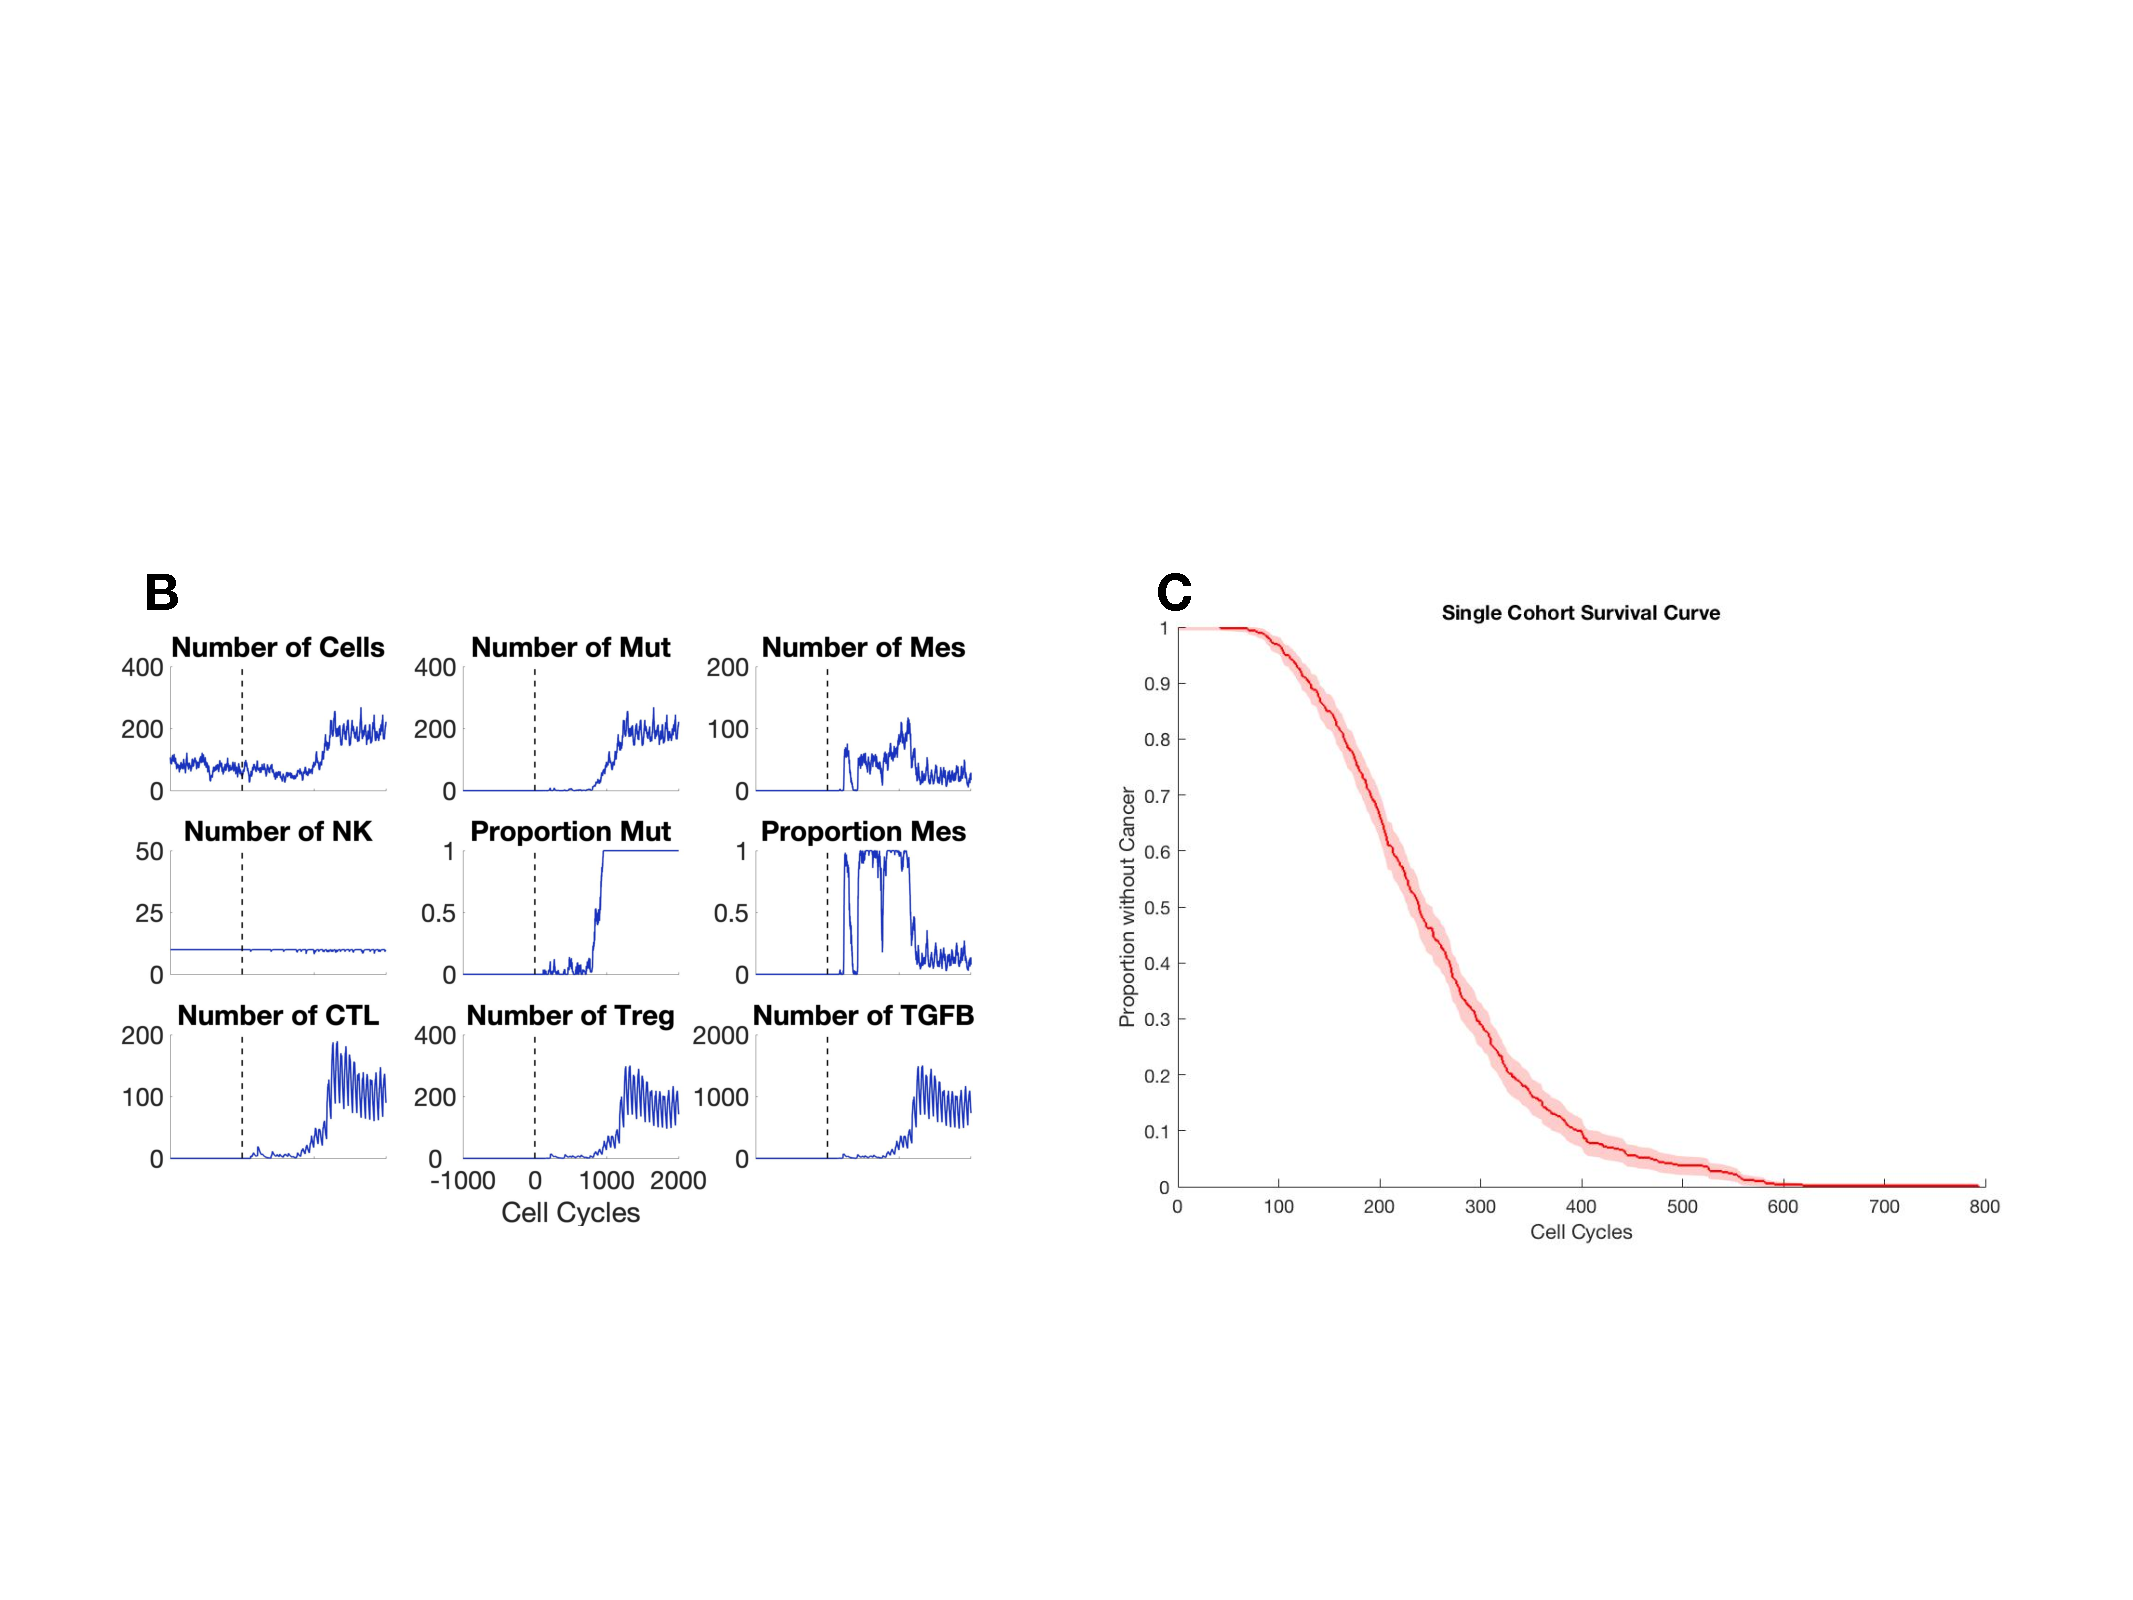
\includegraphics[width=1\textwidth]{../Figs/Figure1/SI_fig1.pdf}}
\caption[Fig. 1BC without targeting premalignant cells]{
A. Single patient trajectory without immune cells targeting premalignant cells. Compare to Fig. 1B. B. Sample cohort survival curve without immune cells targeting premalignant cells. Compare to Fig. 1C.
}
\label{fig:1_first}
\end{figure}

\begin{figure}
\center
{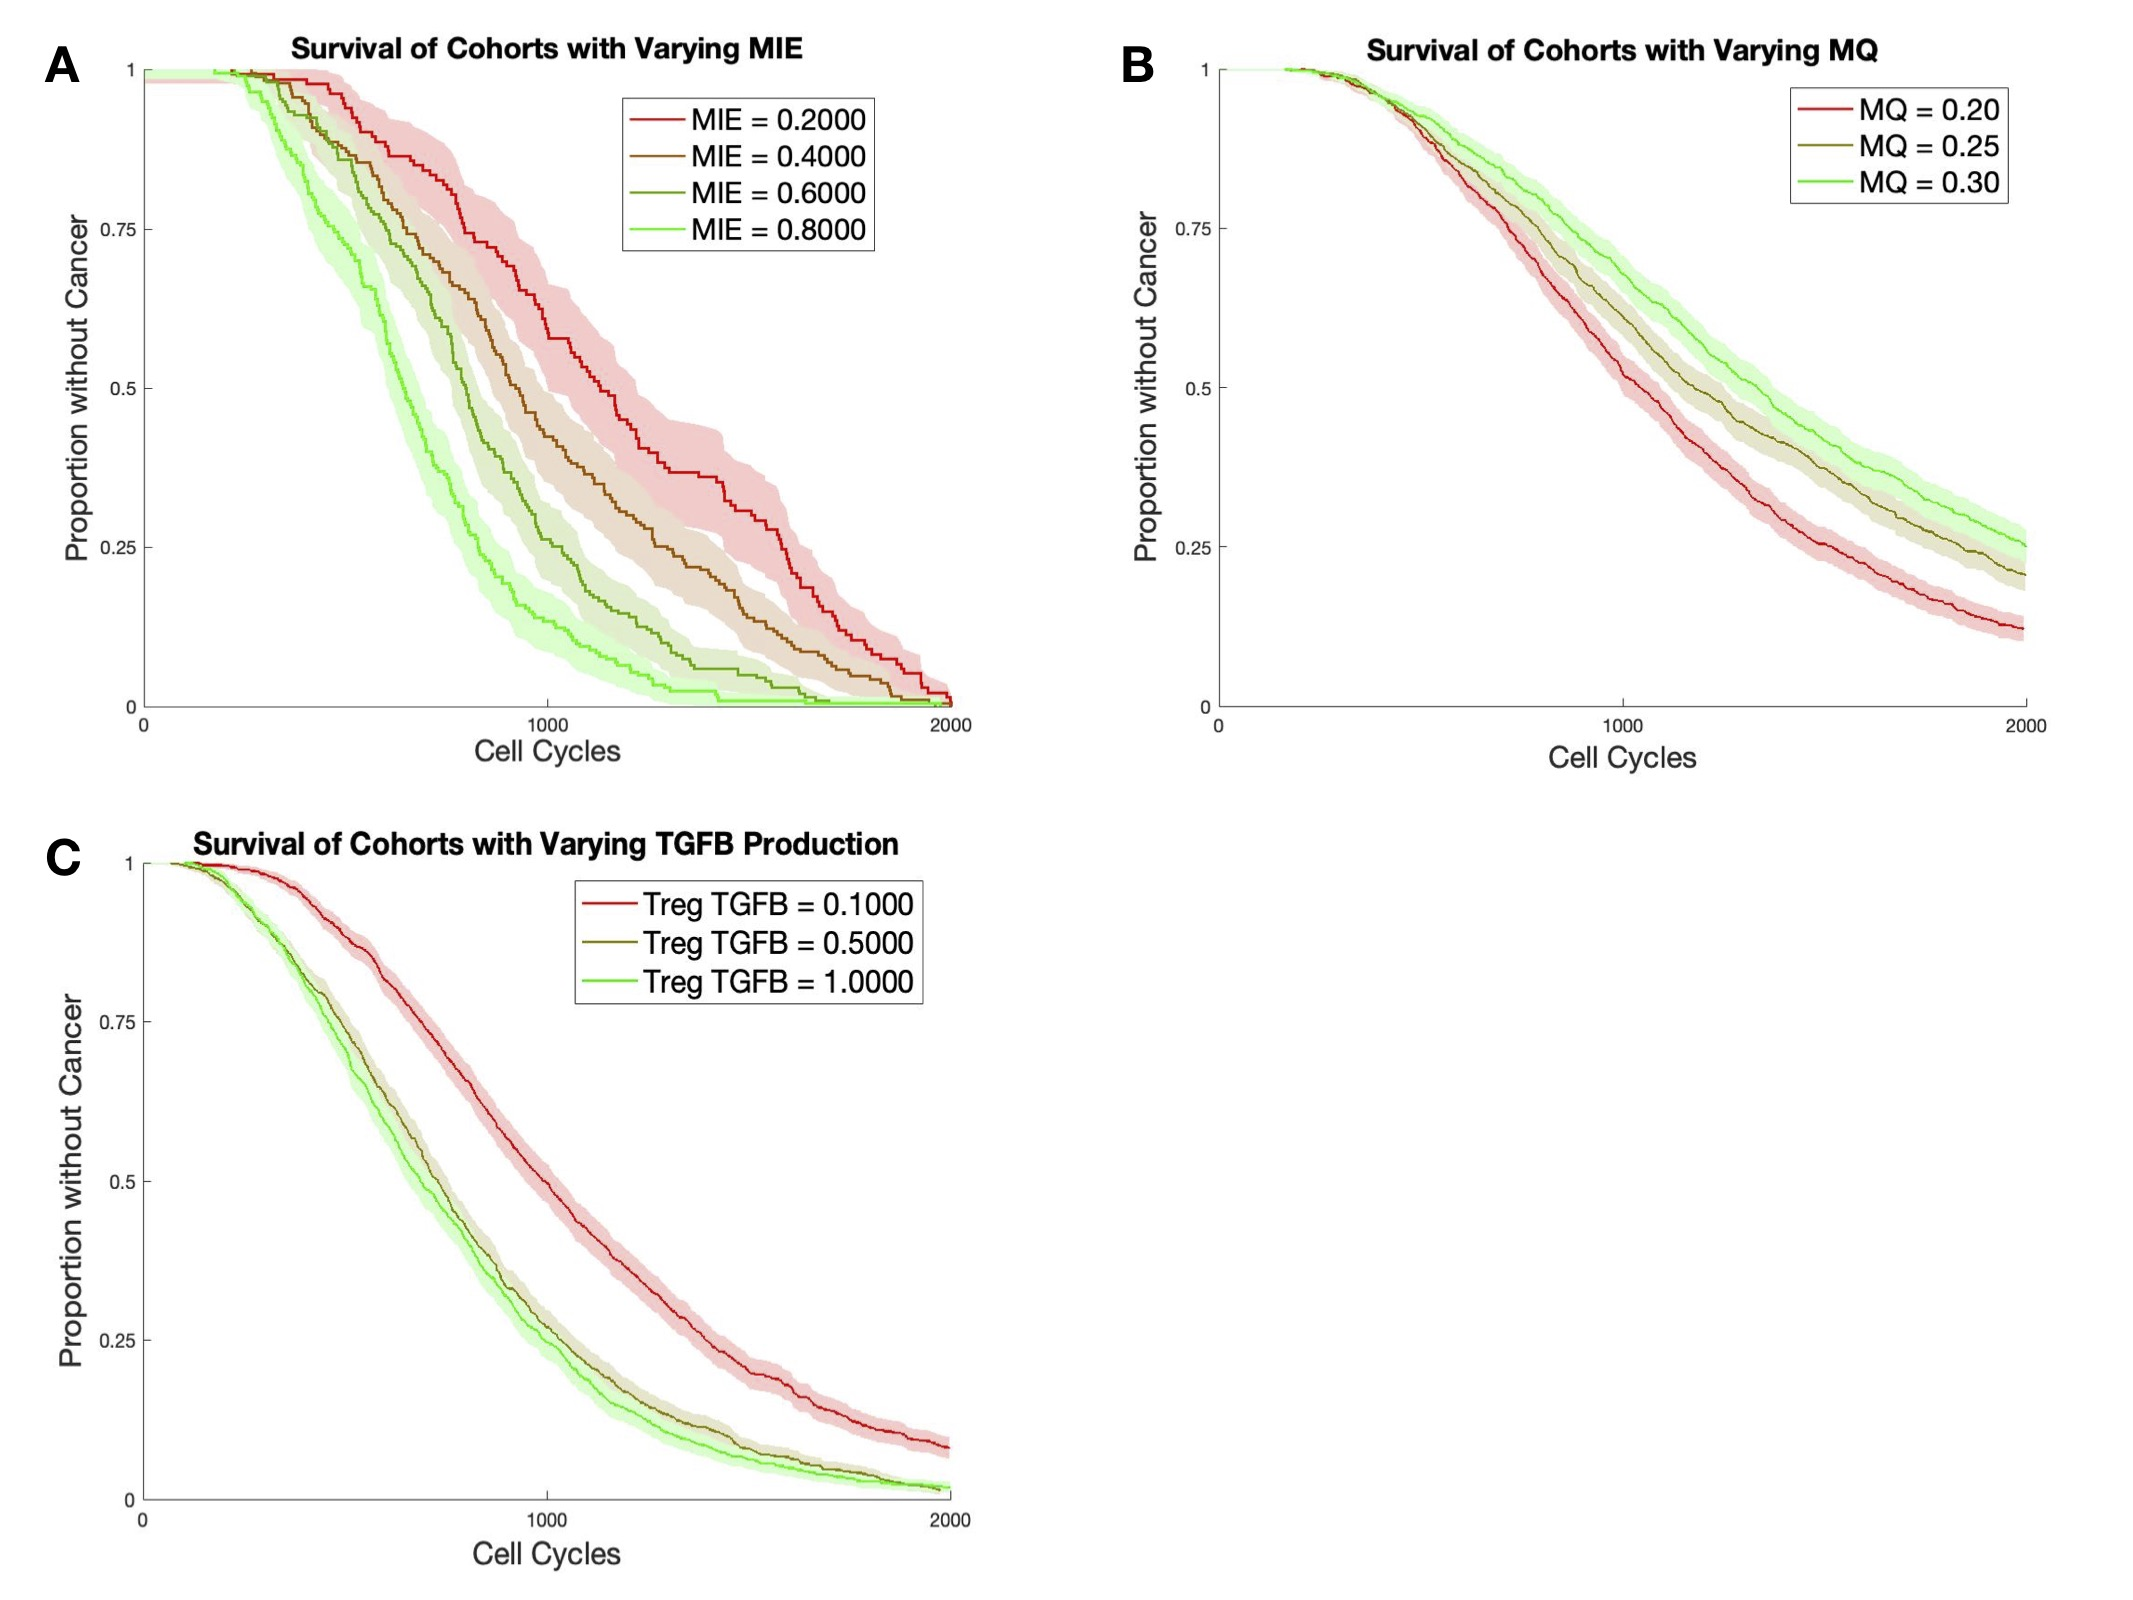
\includegraphics[width=0.65\textwidth]{../Figs/Figure2/Figure2.jpg}}
\caption[Fig. 2 without targeting premalignant cells]{
Morris-OAT global sensitivity without immune cells targeting premalignant cells. Compare to Fig. 2.
}
\label{fig:2_first}
\end{figure}

\begin{figure}
\center
{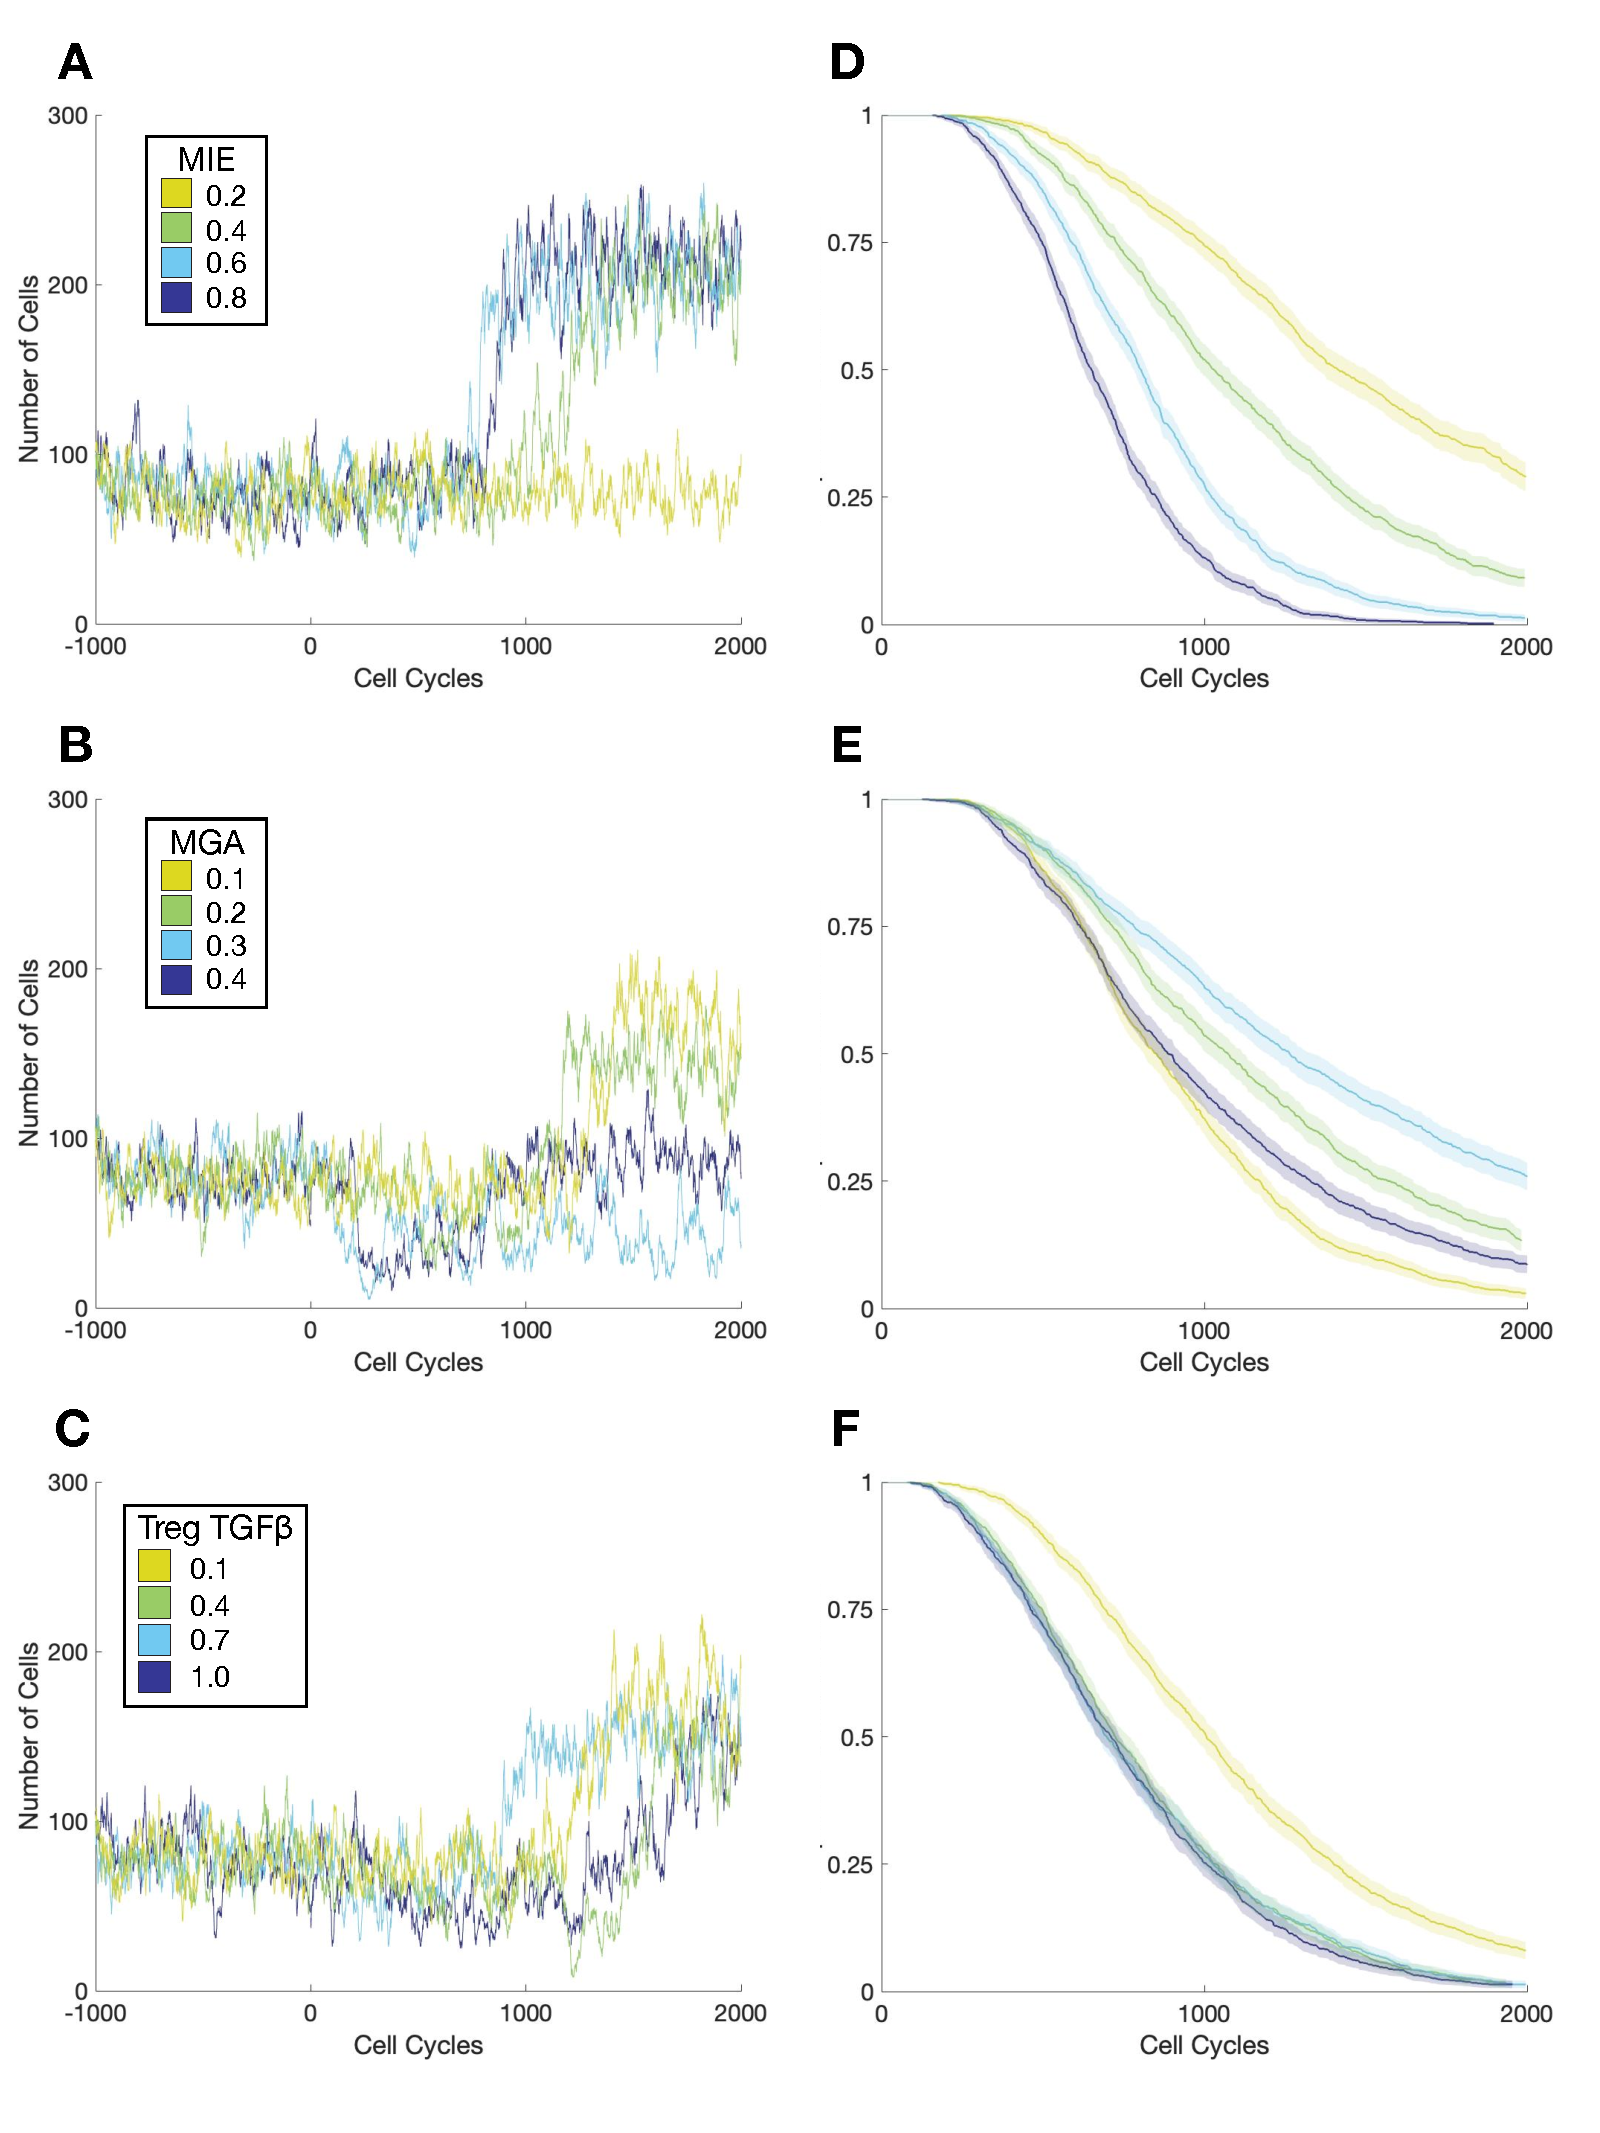
\includegraphics[width=0.65\textwidth]{../Figs/Figure3/Outdated/Figure3_first.pdf}}
\caption[Fig. 3 without targeting premalignant cells]{
Effects of mesenchymal tumor cell properties on the Time to Cancer without immune cells targeting premalignant cells. Compare to Fig. 3.
}
\label{fig:3_first}
\end{figure}

\begin{figure}
\center
{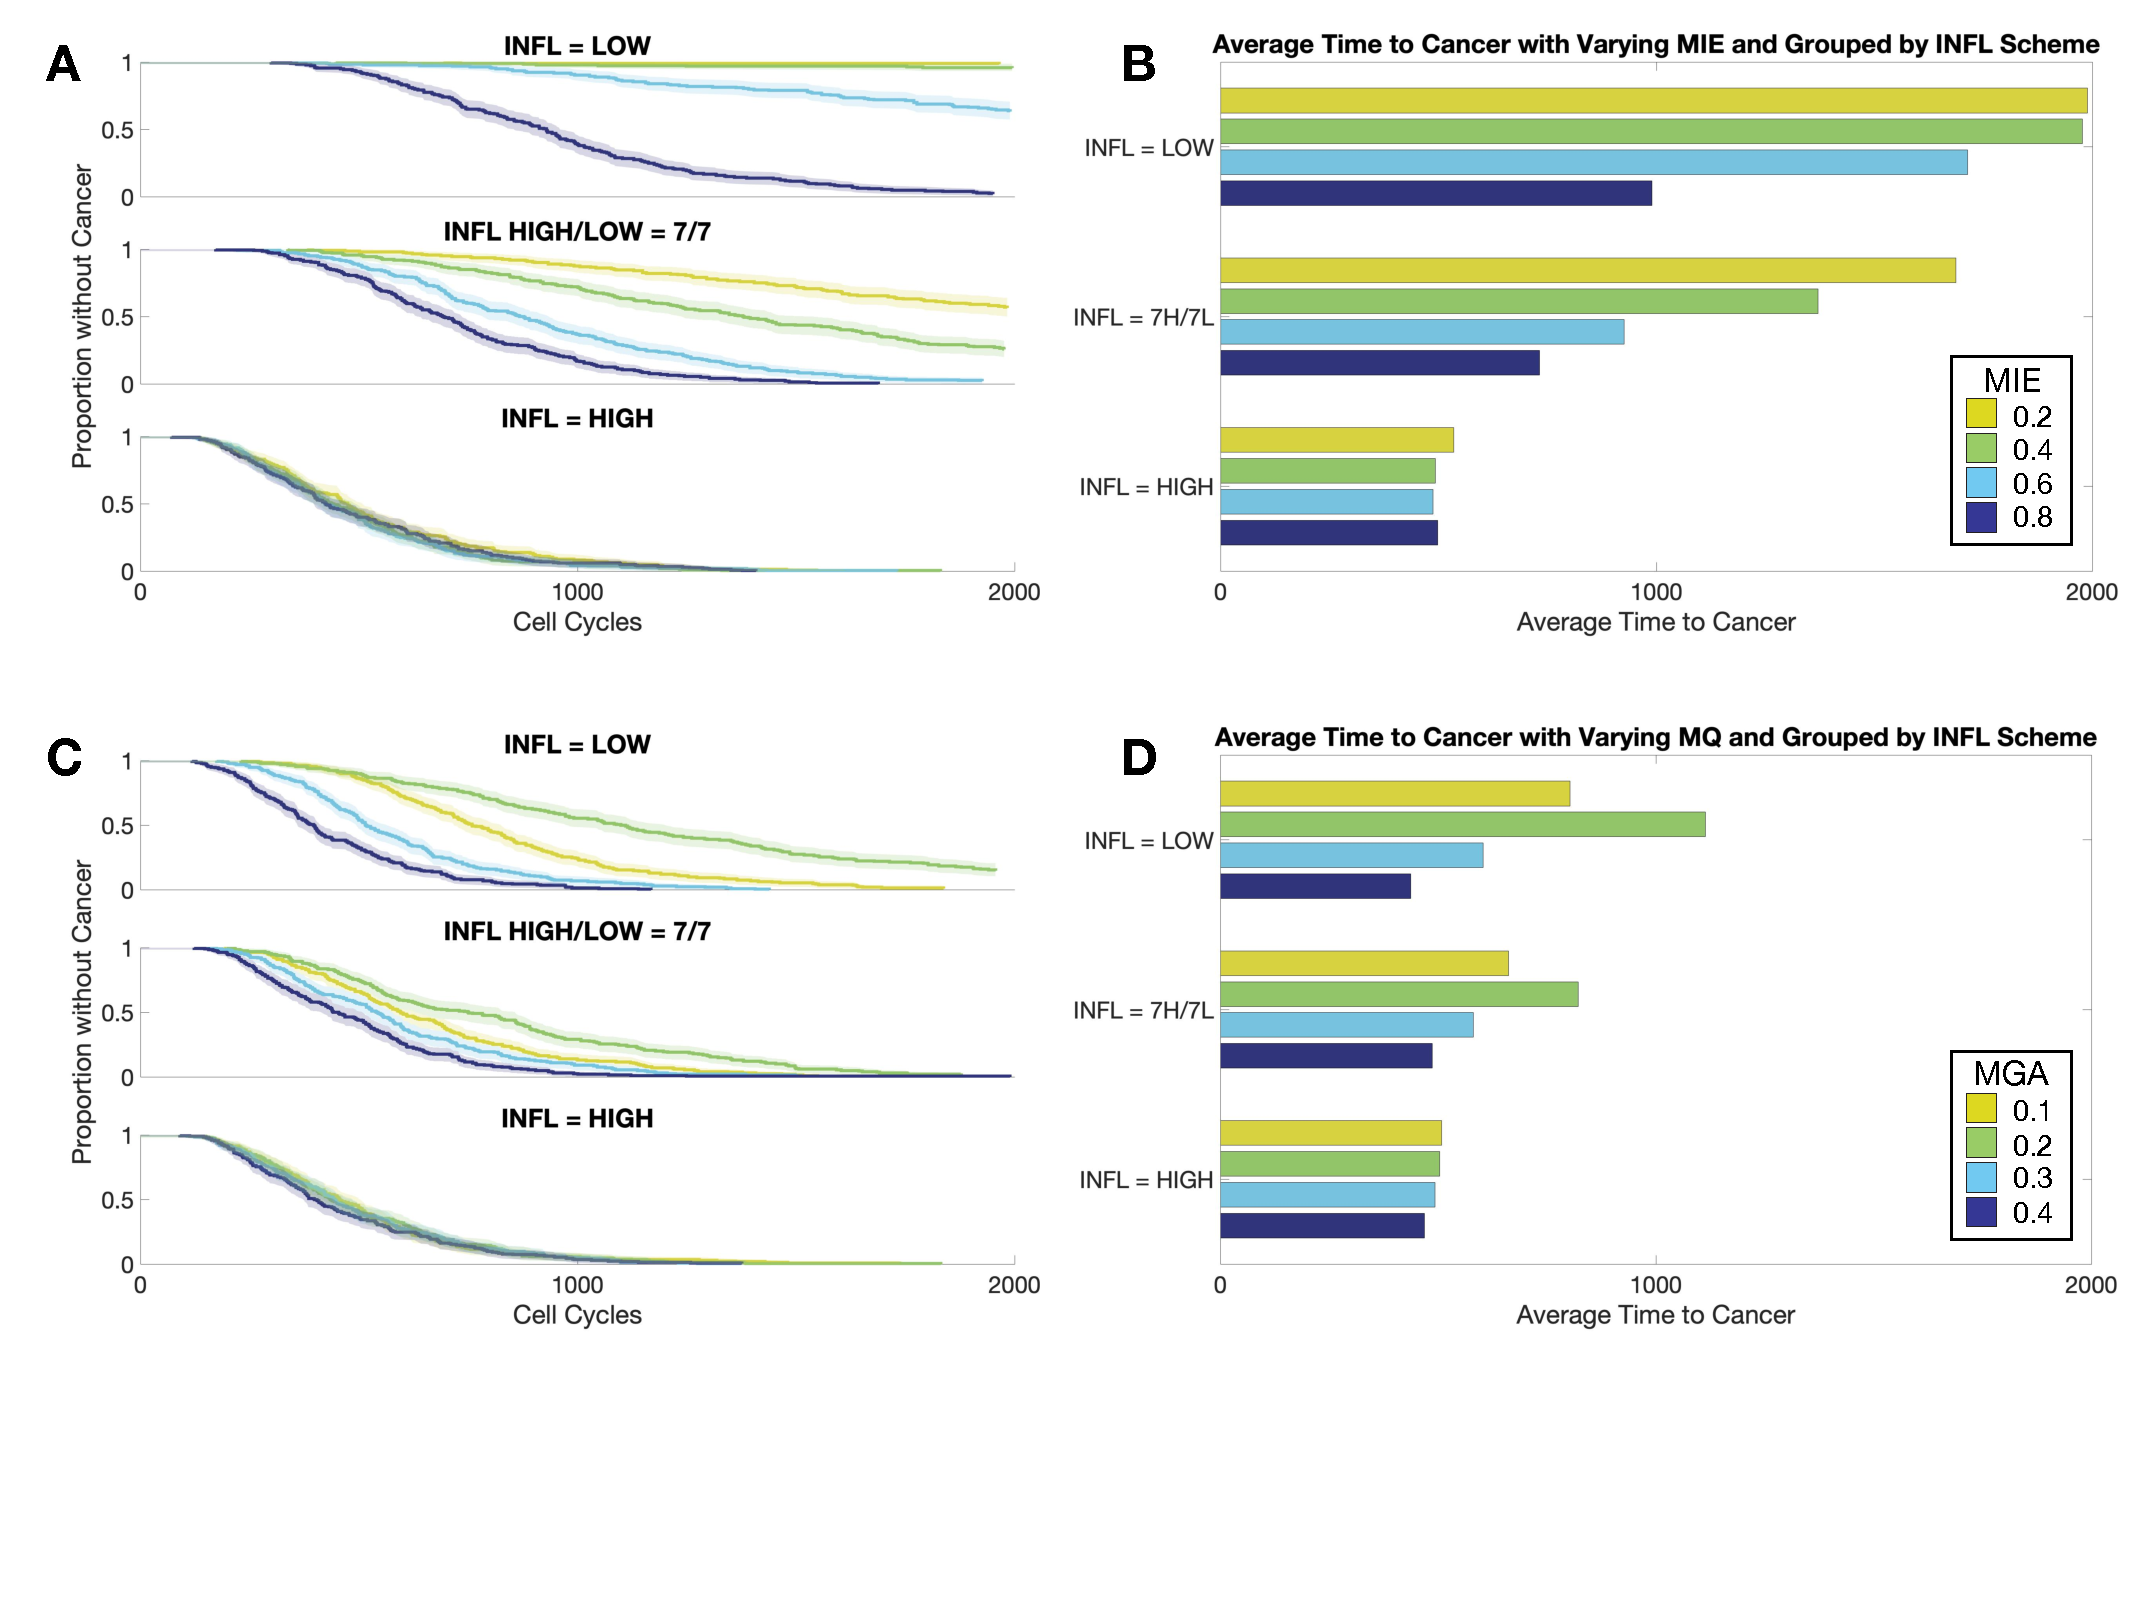
\includegraphics[width=0.65\textwidth]{../Figs/Figure4/Figure4_first.pdf}}
\caption[Fig. 4 without targeting premalignant cells]{
Effects of inflammation on the Time to Cancer without immune cells targeting premalignant cells. Compare to Fig. 4.
}
\label{fig:4_first}
\end{figure}

\begin{figure}
\center
{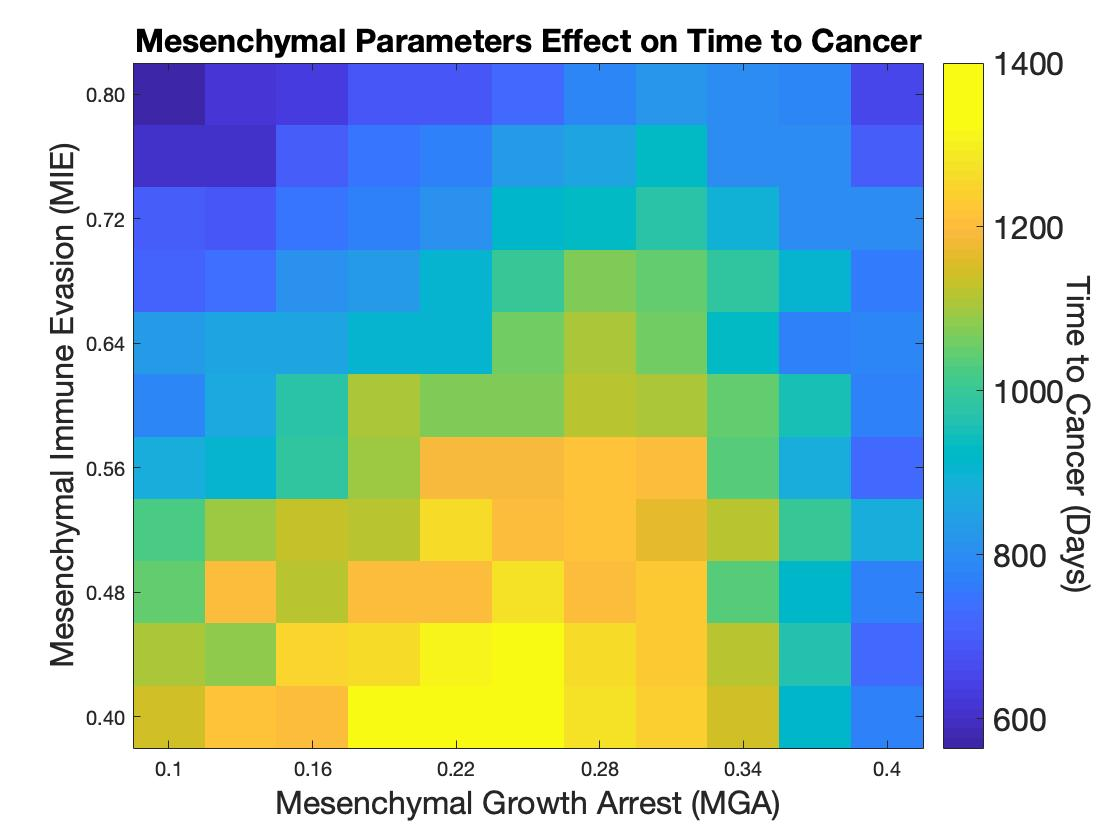
\includegraphics[width=0.65\textwidth]{../Figs/Figure5/MIEvsMGA_bigcbar.jpg}}
\caption[Fig. 5 without targeting premalignant cells]{
Summary of the contrasting effects of MIE and MGA on Time to Cancer without immune cells targeting premalignant cells. Compare to Fig. 5.
}
\label{fig:5_first}
\end{figure}



\begin{figure}
\center
{\includegraphics[width=0.65\textwidth]{../Figs/Figure6/SKCM.pdf}}
\caption[SKCM TCGA Data Analysis]{A. K-means clustering of SKCM using gene ontology terms indicative of EMT and inflammation signatures ($k=2$).
B. Survival plots corresponding to the clustering on EMT and inflammation.
C. K-means clustering of SKCM using gene ontology terms indicative of an EMT signature ($k=2$).
D. Survival plots corresponding to the clustering on EMT.
E. K-means clustering of SKCM using gene ontology terms indicative of inflammation ($k=2$).
F. Survival plots corresponding to the clustering on inflammation.}
\label{fig:SKCM}
\end{figure}

\begin{figure}
\center
{\includegraphics[width=0.65\textwidth]{../Figs/Figure6/LIHC.pdf}}
\caption[LIHC TCGA Data Analysis]]{A. K-means clustering of LIHC using gene ontology terms indicative of EMT and inflammation signatures ($k=2$).
B. Survival plots corresponding to the clustering on EMT and inflammation.
C. K-means clustering of LIHC using gene ontology terms indicative of an EMT signature ($k=2$).
D. Survival plots corresponding to the clustering on EMT.
E. K-means clustering of LIHC using gene ontology terms indicative of inflammation ($k=2$).
F. Survival plots corresponding to the clustering on inflammation.}
\label{fig:LIHC}
\end{figure}

\begin{figure}
\center
{\includegraphics[width=0.65\textwidth]{../Figs/Figure6/LUAD.pdf}}
\caption[LUAD TCGA Data Analysis]{A. K-means clustering of LUAD using gene ontology terms indicative of EMT and inflammation signatures ($k=2$).
B. Survival plots corresponding to the clustering on EMT and inflammation.
C. K-means clustering of LUAD using gene ontology terms indicative of an EMT signature ($k=2$).
D. Survival plots corresponding to the clustering on EMT.
E. K-means clustering of LUAD using gene ontology terms indicative of inflammation ($k=2$).
F. Survival plots corresponding to the clustering on inflammation.}
\label{fig:LUAD}
\end{figure}

\end{document}